\bghdr{images/fond-mac}

%\begin{center}
%
\includegraphics{images/logo_Mac}
%\end{center}



\subsection{Configuration sous Mac OS X}

La configuration est détaillée pour Mac OS 10.5 (\app{Leopard}). %et encore un peu pour Mac OS 10.4 (Tiger).
Afin de connaître la version que tu utilises, va dans le \menu{menu Pomme} puis sélectionne \menu{A propos de ce Mac}.

\subsubsection{Configuration IP}

\flimage{images/mac_prefs_icone}{0.07}{l}
 \app{Préférences Réseau}, accessible depuis l'article de menu \menu{Préférences système} du menu \menu{Pomme}, permet de configurer la connexion au réseau. Par ailleurs, si au démarrage un assistant te propose de configurer ton réseau, refuse et utilise la procédure du BR. En effet, le réseau nécessite une configuration particulière  l'X, plus complexe que celle effectuée par cet assistant.


\noindent
  \begin{figure*}[p]
    \begin{center}  
     % \subfloat[Tiger]{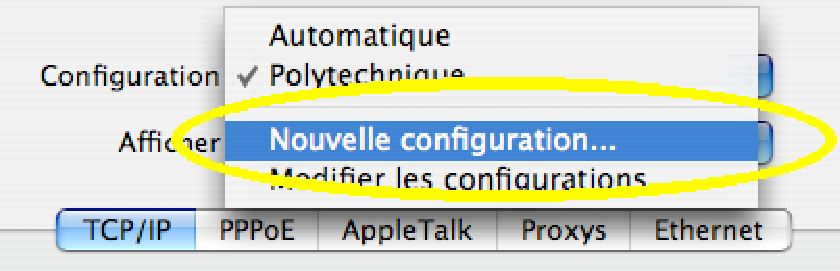
\includegraphics[width=0.47\textwidth]{images/mac_nouvelle_config} } 
     % \hfill
      \subfloat[Créer une nouvelle configuration réseau]{ 
      \begin{minipage}{0.43 \textwidth}\begin{flushleft}
      {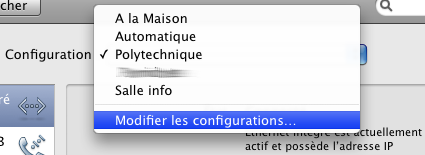
\includegraphics[width=0.96\textwidth]{images/mac_nouvelle_config_leopard_1}}\\ \vspace*{2cm}
      {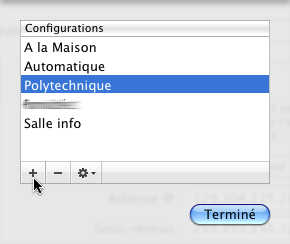
\includegraphics[width=0.96\textwidth]{images/mac_nouvelle_config_leopard_2}} 
 		\end{flushleft}  \end{minipage}
 		 } 		
 		\subfloat[Configuration de l'interface réseau \emph{Ethernet}, de l'adresse IP et du \emph{proxy}]{ 
 		 \begin{minipage}{0.43 \textwidth}\begin{flushright}
 		{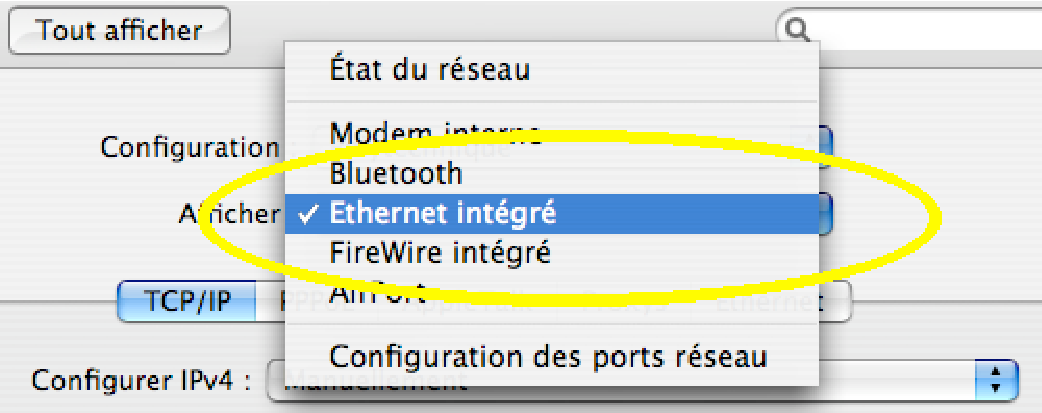
\includegraphics[width=0.96 \textwidth]{images/mac_config_ethernet}} \\ 
 		{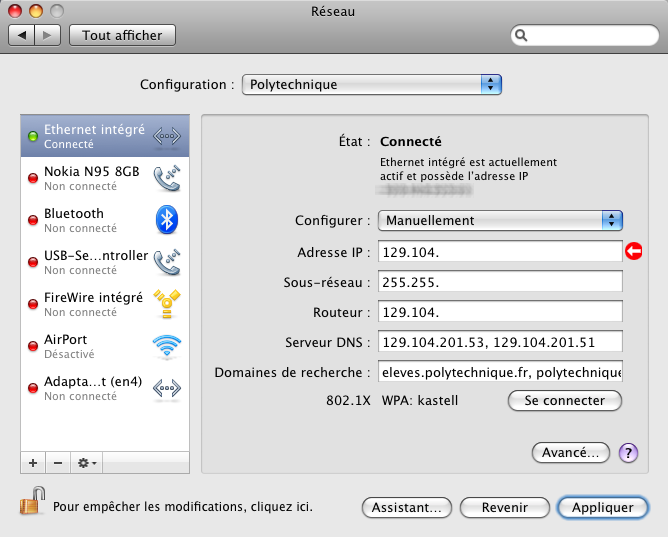
\includegraphics[width=0.96 \textwidth]{images/mac_config_ip_leopard}} \\
 		{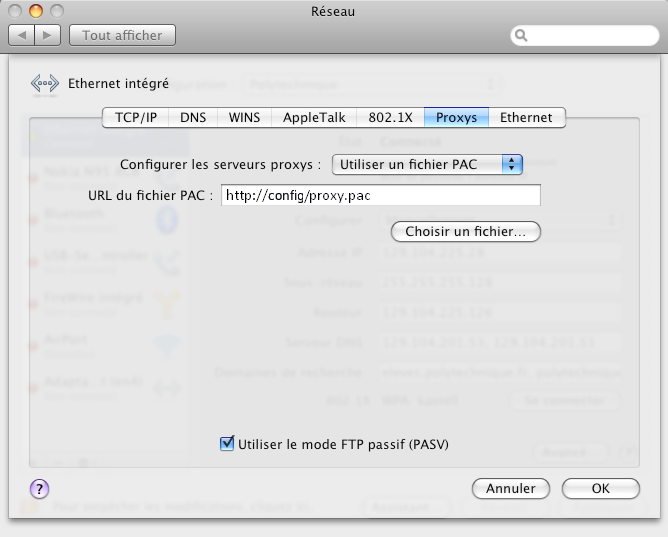
\includegraphics[width=0.96 \textwidth]{images/mac_config_proxy_leopard}}
\end{flushright}
 		\end{minipage}
 		 	\label{config:mac:ip:leopard}	}
     	 \caption{Créer une nouvelle configuration réseau}

    \end{center}
  \end{figure*}

La gestion des configurations réseau de Mac OS X permet de créer plusieurs configurations et de passer en un clic de l'une  l'autre grâce au sous-menu \menu{Configuration Réseau} du menu \menu{Pomme}. Cela est très pratique pour les machines vouées à être connectées à plusieurs endroits successivement --- les portables par exemple (voir la page~\pageref{wifi} puis la section \emph{Wi-Fi} pour plus de précisions sur le \emph{Wi-Fi}). Commence donc par créer une nouvelle configuration réseau dans le menu déroulant \menu{Configuration}.



Une fois la nouvelle configuration créée, il faut configurer l'interface réseau \emph{Ethernet}.



\app{Leopard} : Dans la colonne de gauche, sélectionne \menu{Ethernet intégré}.

Choisis alors \menu{Configurer IPv4} :% \menu{Manuellement} (\app{Tiger}) ou 
\menu{Configurer} : \menu{Manuellement} (\app{Leopard}). Tu trouveras toutes les valeurs d'adresses IP nécessaires pour la configuration en page \pageref{calcul_ip} ou en te reportant aux captures d'écran~\ref{config:mac:ip:leopard}. Si une partie d'adresse IP est blanche sur ces captures, c'est qu'elle t'est personnelle et que tu dois la calculer !


  
  

%\imageref{images/mac_config_ip_leopard}{0.4}{Configuration IP (Leopard)}{!ht}{config:mac:ip:leopard}}


Pour avoir accès à Internet, il faut aussi configurer le \emph{proxy}.

\app{Leopard} : Clique sur le bouton \menu{Avancé...} puis sur l'onglet \menu{Proxys}.


\app{Mac OS X 10.3.3 et supérieur} :  choisis l'option \menu{Configuration automatique de proxy}. Pour Mac OS X 10.3 à 10.3.2, n'oublie pas une fois que tu as le réseau de faire la mise à jour de ton système, pour pouvoir configurer de façon automatique le \emph{proxy}.

\app{Mac OS X 10.3.2 et inférieur} : il te faut spécifier tous les
\emph{proxies} manuellement, et mettre \server{kuzh.polytechnique.fr}, port \server{8080}.


N'oublie pas d'activer le mode passif pour les transferts en FTP, en cochant la case comme dans la capture.



  
\subsubsection{Configuration \emph{Wi-Fi} Bataclan}
Pour configurer le \emph{Wi-Fi} au Bataclan, il faut tout d'abord que tu télécharges  le certificat sur \urllink{http://wifi/certificats.html}.
Dans l'onglet \menu{Airport}, choisis comme réseau \menu{kastell} puis dans l'onglet \menu{Avancé}, choisis \menu{802.1W} et saisis ton \emph{login} poly (seulement 8 caractères max) et votre mot de passe \server{Frankiz}. N'oublie pas de cocher la case TTLS comme dans la capture.

\begin{figure*}[p]
    \begin{center}
      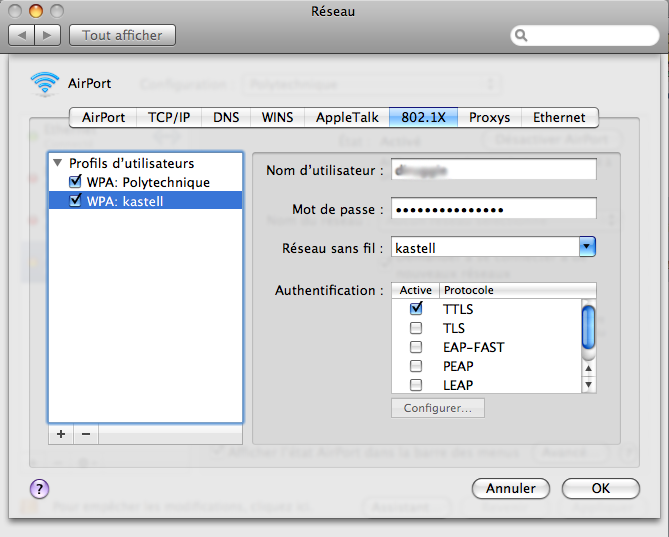
\includegraphics[width=0.4\textwidth]{images/mac_config_wifi.png} 
      \caption{Configurer le \emph{Wi-Fi} du Bataclan}
    \end{center}
  \end{figure*}

%cette section est redondante un peu avec celle du \emph{Wi-Fi}

\subsubsection{Configuration antivirus}

Bien qu'il soit important de maintenir ton système à jour, un antivirus est pour l'instant tout à fait superflu sur Mac, puisqu'aucun virus fonctionnel n'a encore vu le jour. Attention cependant, n'ouvre pas des fichiers dont tu ne te sois pas assuré de la provenance, et essaie de te tenir au courant des actualités concernant les failles des applications que tu utilises.



\subsubsection{Configuration web}

\flimage{images/mac_safari_icone}{0.07}{l}
\app{Safari}, le navigateur web d'Apple, est maintenant compatible avec la majorité des sites \emph{web}. Tu peux donc t'en servir au quotidien, en faisant appel à \app{Firefox} ou \app{Camino} pour les sites récalcitrants. Un conseil : pense à activer le blocage des fenêtres \emph{pop-up} (dans le menu \menu{Safari}). \app{Safari} peut aussi servir de client RSS (voir plus bas).\\


\subsubsection{Configuration \emph{mail}}
\flimage{images/mac_mail_icone}{0.07}{l} \app{Mail} : un client \emph{mail} offrant les fonctionnalités classiques d'un bon client : recherche instantanée, filtre antispam, règles de tri automatique des \emph{mails}, regroupement des \emph{mails} correspondant à une même discussion.

Au premier lancement, \app{Mail} te demandera de remplir les informations concernant ton compte \emph{mail} sur \server{poly}, il suffit de le remplir avec les données suivantes :
\begin{description}
  \item[Nom complet] ton nom !
  \item[Adresse électronique] de la forme \mail{prenom.nom@polytechnique.edu}
  \item[Serveur de réception] \server{poly.polytechnique.fr}
  \item[Type de compte] \menu{POP}
  \item[Nom d'utilisateur] ton \emph{login} \server{poly} (les huit premières lettres de ton nom en général)
  \item[Mot de passe] ton mot de passe \server{poly}
  \item[Serveur d'envoi (SMTP)] \server{poly.polytechnique.fr} ou \server{ssl.polytechnique.org}
\end{description}

Si tu as déjà créé un compte précédemment, il faut aller dans les \menu{Préférences} (accessibles depuis le menu \menu{Mail}), onglet \menu{Comptes}, pour créer un autre compte en cliquant sur la case \menu{+}.

N'oublie pas de cocher \menu{Activer le cryptage SSL} dans l'onglet \menu{Avancé}, port 995. Tu souhaiteras alors certainement installer le certificat de sécurité de \server{poly} (tu le trouveras sur \urllink{http://poly/}). Une fois que tu as téléchargé le certificat, ouvre le fichier \menu{.CRT} obtenu, et dans \app{Trousseau d'accès}, installe-le dans %\menu{X509Anchors} (Tiger) ou 
\menu{session} (Leopard).

Cette configuration marche pour accéder à ses mails depuis l'intérieur de l'X mais aussi de l'extérieur, sans rien changer. En revanche tu ne peux pas envoyer de \emph{mails} depuis l'extérieur , car le serveur \server{poly} ne le permet pas. Nous te conseillons vivement d'utiliser le serveur SMTP \server{polytechnique.org} et de regarder la configuration proposée par \urllink{Polytechnique.org}. Celle-ci permet d'envoyer des \emph{mails} sûrs à l'extérieur de l'école sans modifier ta configuration par la suite. Tu peux ajouter ce SMTP dans l'onglet \menu{Comptes} des \menu{Préférences} de \emph{mail} et régler dans l'onglet \menu{Avancés} comme dans la capture.

\begin{figure*}[!hl]
    \begin{center}
	      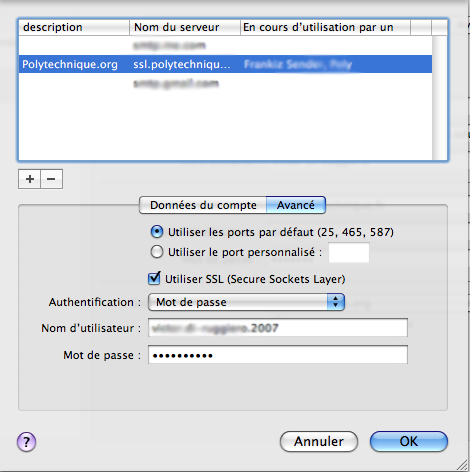
\includegraphics[width=0.4\textwidth]{images/mac_config_smtp_poltechnique.png} 
      \caption{Configurer le serveur SMTP \server{Polytechnique.org}}
    \end{center}
  \end{figure*}



Le LDAP ne fonctionne pas à l'heure actuelle avec \app{Mail} (mars 2009) sous \app{Leopard}, contrairement aux  autres systèmes d'exploitation (fonctionne cependant avec \app{Thunderbird}).
%\subsuEnfin, tu peux disposer dans \app{Mail} de l'annuaire de l'École, mis à disposition par la DSI. Pour cela, va dans les \menu{Préférences} de Mail,
%puis dans la rubrique \menu{Rédaction} et clique sur \menu{Configurer LDAP\ldots}. Tu peux ensuite utiliser le bouton \menu{+} pour ajouter un
%serveur, et remplir la fenêtre comme sur la capture.

%\imagepos{images/mac_config_ldap}{0.6}{Configurer l'annuaire}{!ht}
%bsection{Logiciels additionnels}


Les logiciels suivants sont utiles pour utiliser avec Mac OS X les services proposés sur le réseau ; ils sont téléchargeables sur \server{frankiz}, dans la rubrique \menu{Télécharger}, \menu{Mac}.

\pagebreak

\subsubsection{Configuration \emph{news}}

\flimage{images/mac_thunderbird_icone}{0.07}{l} 
\app{Thunderbird} : un client \emph{news} permettant d'accéder aux forums de discussion des élèves (voir page~\pageref{newsgroups} pour les détails sur \server{frankiz}), mais aussi à ceux de \server{usenet} grâce au serveur \server{polynews.polytechnique.fr}. Il est très proche d'\app{Outlook Express} dans son esprit. Dans la même catégorie, il existe \app{MacSOUP}, \app{Unison} ou encore \app{MT-NewsWatcher}. La configuration se fait de la même manière.

Au premier lancement, l'application te propose d'importer les paramètres depuis une autre application. Clique sur \menu{Suivant}. Tu peux alors choisir quel type de compte tu veux configurer (tu remarqueras que tu peux aussi créer un compte courrier électronique, et un compte RSS). Sélectionne \menu{Compte forums de discussion} et clique sur \menu{Suivant}. Entre alors les informations suivantes :

\begin{description}
  \item[Votre nom] ton nom ou ton pseudo
  \item[Adresse de courrier] \mail{prenom.nom@polytechnique.edu}
  \item[Serveur de forums] \server{frankiz}
  \item[Nom du compte] News Frankiz
  \item[Nom d'utilisateur] ton \emph{login }poly (les huit premières lettres de ton nom en général)
  \item[Serveur d'envoi (SMTP)] \server{poly.polytechnique.fr} ou \server{ssl.polytechnique.org}
\end{description}


Pour t'abonner à des groupes de discussion, il te suffit de sélectionner le compte \menu{News Frankiz} dans la fenêtre \menu{Dossiers} de \app{Thunderbird}, puis de cliquer sur \menu{Gérer les abonnements aux groupes de discussion}. Tu pourras ensuite sélectionner les forums qui t'intéressent parmi la liste proposée. Reporte-toi à la page \pageref{newsgroups} pour plus d'infos sur les \emph{newsgroups} auxquels t'abonner !

\subsubsection{Firefox}
Un point particulier pour la configuration du \emph{proxy} de Firefox : dans \menu{Préférences}, \menu{Avancé}, \menu{Réseau}, clique sur \menu{Paramètres} et choisis \emph{Adresse de configuration de proxy automatique} : \urllink{http://frankiz/proxy.pac}



\subsubsection{FTP}

\flimage{images/mac_cyberduck_icone}{0.07}{l} \app{Cyberduck} : un client FTP très simple à utiliser mais performant. Il te permettra d'aller télécharger des fichiers sur les serveurs FTP des autres élèves.
 %Il existe aussi \app{Transmit} (partagiciel), ou encore \app{Fugu}, que certains préfèrent.
Pour se connecter à un serveur, il suffit de taper son nom (exemple : \urllink{jtx}) dans le cadre \menu{Connexion rapide} et appuyer sur Entrée.\\
Tu verras rapidement que tout le monde à l'X possède un serveur FTP afin de partager les différents projets, les films du JTX, ses photos, etc. Donc il est quasiment indispensable que tu en installes un. Nous te conseillons \app{PureFTPd Manager}, qui dispose d'une interface très facile à utiliser (même pour un débutant) et en même temps de fonctionnalités avancées très puissantes. Tu trouveras le détail de sa configuration sur le WikiX.

\subsubsection{Autres logiciels utiles}

Les logiciels cités ici sont téléchargeables sur \server{frankiz}, rubrique \menu{Télécharger}, \menu{Mac}, \menu{Réseau}.

\flimage{images/mac_qrezix_icone}{0.07}{l} \noindent\app{qRezix} : en deux mots, c'est un programme développé par le BR pour faciliter la vie sur le réseau. Tu peux le récupérer dans la partie Mac de \xshare.

\noindent Pour plus de détails, voir le paragraphe consacré à qRezix à la page \pageref{qrezix}.

\noindent \app{Leopard} : le pare-feu se règle application par application, tu n'auras qu'à répondre \menu{Autoriser} lorsqu'il te demandera si tu veux \menu{Autoriser les connexions entrantes}.

%\noindent  \app{Tiger} : Attention, si ton \emph{firewall} est activé, tu dois ouvrir les ports 5050, 5053 et 5055 en TCP. Pour cela va dans \app{Préférences Système}, dans le module \menu{S\'ecurit\'e}, onglet \menu{Coupe-feu}. S'il est écrit \menu{Coupe-feu activé}, clique le bouton \menu{Nouveau} et remplis la boîte de dialogue comme sur la capture d'écran ci-dessous pour ouvrir les ports.

%\imagepos{images/mac_firewall}{0.5}{Ouvrir les ports pour \app{qRezix} (Tiger)}{!ht}

%\flimage{images/mac_conversation_icone}{0.1}{l}
%\noindent\app{Colloquy}, un client IRC dans le même esprit qu'\app{iChat}. Il dispose d'une interface très simple ne nécessitant pas de connaître les commandes IRC. Tu peux te reporter à la page \pageref{irc} pour plus d'infos sur l'IRC. \app{X-Chat Aqua} est un autre client IRC, plus riche en fonctionnalités, mais moins agréable à utiliser. \\

%\flimage{images/mac_netnewswire_icone}{0.1}{l}
%\noindent\app{NetNewsWire} est la référence des clients RSS sur Mac, et est maintenant gratuit. Dans le même genre, on peut citer \app{Vienna}, un client RSS open source, dont le développement actif est prometteur. Les flux RSS permettent d'agréger dans un seul logiciel des informations en provenance de nombreux sites web, qui peuvent provenir de forums de discussions, de mises à jour de logiciels, d'informations internationales\dots \\ \\

%\flimage{images/mac_fink_icone}{0.1}{l}
\noindent\app{Fink} est la manière la plus simple d'installer sur Mac OS X nombre de logiciels issus du monde Unix (Linux par exemple). Grâce à lui, tu pourras installer les mêmes logiciels que dans les salles informatiques. Par exemple, tu pourras installer Scilab sans trop de peine\dots La configuration nécessaire se trouve sur \urllink{http://frankiz/binets/reseau/Miroir\_Fink}. \\ 

\flimage{images/logo_Windows}{0.1}{l}
\noindent \app{Windows et les Mac Intel} : Maintenant il est possible d'installer Windows grâce à \app{Boot Camp}, livré avec \app{Leopard}. Cela te permettra de profiter des quelques applications du monde PC qui valent le coup tout en gardant ton Mac. Tu peux également virtualiser Windows (utiliser Windows en utilisant en même temps Mac OS) grâce à \app{VMware Fusion}, \app{VirtualBox} ou \app{Parallels Desktop}. Le  défaut de cette solution est que tu n'as pas d'accélération 3D, donc pour les jeux il te faudra redémarrer. Ces deux logiciels sont disponibles en version d'essai sur leurs sites \emph{web} respectifs. \`A toi de choisir !
Mais vérifie tout de même que tu as bien un processeur Intel (\menu{Pomme} puis sélectionne \menu{À propos de ce Mac}).

\pagebreak
